\documentclass[12pt]{article}
\usepackage{setspace}
\usepackage{fullpage}
\usepackage{graphicx}
\usepackage{subfigure}
\usepackage{yhmath,wasysym}
\setlength{\parindent}{0em}
\setlength{\parskip}{0.85em}
\setstretch{1.2}
\def\bmath#1{\mbox{\boldmath$#1$}}

\usepackage{color}
\definecolor{darkblue}{rgb}{0,0,0.4}
\usepackage[colorlinks=true,citecolor=black,linkcolor=darkblue,
urlcolor=darkblue,bookmarks=false,bookmarksopen=false,
pdfpagemode=None,pdfstartview=FitH]{hyperref}
\newcommand*{\DOT}{.}

% \title{Notes on Elasticity} %
% \author{Ju Li, Department of Materials Science and Engineering, %
% University of Pennsylvania, Philadelphia, PA 19104, USA} %
% \date{\today} %

\begin{document}
\bibliographystyle{unsrt}

\newcommand{\URL}[1]{\href{#1}{#1}} 

\renewcommand\refname{References \\ ({\small
\URL{http://mt.seas.upenn.edu/Stuff/e/Notes/Paper/}
})}

% \maketitle %
\centerline{\LARGE\bf Notes on Transformation Elasticity} 

\centerline{\large\bf Ju Li, University of Pennsylvania, Sept. 27, 2008}

\section{Inhomogeneous Elasticity Solver}

Given an original supercell ${\bf x}={\bf s}{\bf H}_0$,
${\bf s}\in[0,1)$, we would like to solve the following problem:
\begin{equation}
 F^{\rm el}[{\bf H}, \bmath{\epsilon}^0({\bf x})] \;\equiv\; 
\min_{{\bf u}({\bf x})} 
F^{\rm el}[{\bf u}({\bf x}) | {\bf H}, \bmath{\epsilon}^0({\bf x})]
\end{equation}
\begin{equation}
F^{\rm el}[{\bf u}({\bf x}) | {\bf H}, \bmath{\epsilon}^0({\bf x})] \equiv
 \frac{1}{2}\int d^3{\bf x} c_{ijpq}({\bf x})
 ( \epsilon_{ij}({\bf x}) - \epsilon^0_{ij}({\bf x}) ) 
 ( \epsilon_{pq}({\bf x}) - \epsilon^0_{pq}({\bf x}) )
 \label{ElasticEnergyDefinition}
\end{equation}
where ${\bf u}({\bf x})\equiv {\bf x}^\prime - {\bf x}$, the
difference between the new position ${\bf x}^\prime$ and the old
position ${\bf x}$, and 
\begin{equation}
 \epsilon_{ij}({\bf x}) \;\equiv\; \frac{u_{i,j}+u_{j,i}}{2}.
 \label{LinearElasticStrainDefinition}
\end{equation}
${\bf H}$ is the new supercell: ${\bf H} = {\bf H}_0 ({\bf
I}+\bar{\bmath{\epsilon}})$.  Global rotation of {\bf H} does not
matter anyhow to (\ref{ElasticEnergyDefinition}) to first order in the
global rotation angle, and is therefore ignored in this leading-order
theory.  Note that the untransformed material in ${\bf H}_0$ does not
have to be stress free.  The entire role of ${\bf H}_0$ in the above
is to provide a reference grid.

(\ref{ElasticEnergyDefinition}) is motivated by the following idea
experiment.  One first cuts up the {\em untransformed supercell} ${\bf
H}_0$ into many blocks $d^3{\bf x}$.  Then imagine for instance the
temperature is raised, and phase transformation / plasticity may
induce some blocks to transform to a new state.  Each block, if left
alone (stress free), would like to transform to a new strain state
$\bmath{\epsilon}^0({\bf x})$. Additional local rotation ${\bf R}({\bf
x})$ of the block does not matter to the internal Helmholtz free
energy of {\em this} block \cite{WangLYPW95,LiPhDThesis00}, but needs
to be globally optimized since ${\bf R}({\bf x})$ must be globally
consistent with ${\bf u}({\bf x})$.

Because of the periodic boundary condition, there must be 
\begin{equation}
 {\bf u}({\bf x}+{\bf
h}_0)-{\bf u}({\bf x}) \;=\; {\bf h}_0\bar{\bmath{\epsilon}}
\end{equation}
where ${\bf
h}_0$ is one of the ${\bf H}_0$ edge vectors.  So
\begin{equation}
 \int_0^{{\bf h}_0} d{\bf x}^\prime\cdot 
\frac{d{\bf u}({\bf x}+{\bf x}^\prime)}{d{\bf x}^\prime} 
 \;=\; 
 {\bf h}_0\bar{\bmath{\epsilon}}  \;\;\rightarrow\;\;
 \int d^3{\bf x} \frac{d{\bf u}}{d{\bf x}} =  \det|{\bf H}_0| 
 \bar{\bmath{\epsilon}}.
\end{equation}

Note that $\{\epsilon_{ij}({\bf x})\}$, because of
(\ref{LinearElasticStrainDefinition}), need to satisfy three compatibility
constraints
\begin{equation}
 \epsilon_{ii,jj} + \epsilon_{jj,ii} \;=\; 2 \epsilon_{ij,ij}, 
 \;\;\;\; \forall i\neq j
\end{equation}
which means the $\{\epsilon_{ij}({\bf x})\}$ fields are
not independent fields in the variational functional (the $\{u_i({\bf
x})\}$ fields are). On the other hand, there is no compatibility
constraint \cite{Jagla07} on the stress-free strain fields
$\{\epsilon^0_{ij}({\bf x})\}$, which are ``given'' in the elastic
constant minimization problem.

The functional to be minimized in (\ref{ElasticEnergyDefinition})
represents a quadratic expansion approximation of the Helmholtz free
energy \cite{LiPhDThesis00} around the {\em freely transformed} block.
As such, there should be a conversion factor $\det|d^3{\bf
x}^\prime|/\det|d^3{\bf x}|$ as well as tensor rotation using ${\bf
R}({\bf x})$ to convert the isothermal elastic constant of the
transformed material to $c_{ijpq}({\bf x})$, which is based on the
original volume and observation coordinates.  However, this effect is
higher order, same as the higher-order terms ignored in
(\ref{LinearElasticStrainDefinition}).

Unlike the more general nonlinear formulation of \cite{Jagla07}, the
merit of the quadratic expansion is that
(\ref{ElasticEnergyDefinition}) is quadratic in ${\bf u}({\bf x})$,
whose minimization (in principle at least) entertains a close-formed
solution in the form of a matrix inverse, after real-space
discretization of ${\bf u}({\bf x})$ and representation of
$\nabla^2$-like operators. We have the stress equilibrium equation in
structurally inhomogeneous and elastically inhomogeneous material:
\begin{equation}
 ( c_{ijpq}({\bf x}) 
  ( u_{p,q}({\bf x}) - \epsilon^0_{pq}({\bf x}) ))_{,j} \;=\; 0, 
  \;\;\;\;
  \forall i=1..3
 \label{StressEquilibrium}
\end{equation}


\subsection{Homogeneous Special Case}
\label{sec:HomogeneousSpecialCase}

If the system is elastically homogeneous \cite{WangJK02}, 
$c_{ijpq}({\bf x})=c_{ijpq}^0$, there is
translational symmetry in the problem:
\begin{equation}
 c_{ijpq}^0 ( 
  u_{p,q}({\bf x}) - \epsilon^0_{pq}({\bf x}) )_{,j} \;=\; 0, 
  \;\;\;\;
  \forall i=1..3
\end{equation}
and the inverse can be done in the Fourier space on a ${\bf
k}$-by-${\bf k}$ basis.  We first note that $u_p({\bf x})$ can be
decomposed into a secularly growing component in ${\bf x}$, plus a
periodic component:
\begin{equation}
 u_p({\bf x}) \;\equiv\; {\bf x}\bar{\bmath{\epsilon}} + \tilde{u}_p({\bf x})
\end{equation}
Then stress equilibrium requires that in {\bf k}-space:
\begin{equation}
  -c_{ijpq}^0 k_qk_j \tilde{u}_p({\bf k}) \;=\; 
  ic_{ijpq}^0\epsilon^0_{pq}({\bf k}) k_j
\end{equation}
where 
\begin{equation}
 \tilde{u}_p({\bf k}) \;\equiv\; 
 \int d^3{\bf x} \tilde{u}_p({\bf x})e^{-i{\bf k}\cdot {\bf x}},
 \;\;\;\;
 \tilde{u}_p({\bf x}) \;=\; \frac{1}{\det|{\bf H}_0|}
 \sum_{{\bf k}} \tilde{u}_p({\bf k})e^{i{\bf k}\cdot {\bf x}},
\end{equation}
and similarly $\epsilon^0_{pq}({\bf
k})\leftrightarrow\epsilon^0_{pq}({\bf x})$.  If we define 
symmetric matrix ${\bf C}(\hat{\bf k})$
\cite{WangJK02}
\begin{equation}
 C_{ip}(\hat{\bf k}) \;\equiv\; c_{ijpq}^0 \hat{k}_q\hat{k}_j, \;\;\;\;
 \hat{\bf k}\equiv \frac{{\bf k}}{|{\bf k}|},
 \label{C_Definition}
\end{equation}
the inverse matrix is also real and symmetric: ${\bf \Omega}(\hat{\bf k})\equiv
{\bf C}^{-1}(\hat{\bf k})$.  Let us also define strain-free stress:
\begin{equation}
 \sigma^0_{ij}({\bf x}) \;\equiv\; c_{ijpq}^0\epsilon^0_{pq}({\bf x}), \;\;\;
 \sigma^0_{ij}({\bf k}) \;\equiv\; c_{ijpq}^0\epsilon^0_{pq}({\bf k}),
\end{equation}
then
\begin{equation}
 -|{\bf k}|^2 C_{ip}(\hat{\bf k}) \tilde{u}_p({\bf k}) \;=\; 
 i\sigma^0_{ij}({\bf k})k_j
\end{equation}
and $\tilde{u}_p({\bf k})$ is obtained
explicitly as 
\begin{equation}
 \tilde{u}_p({\bf k}) \;=\; 
 \frac{\Omega_{pi'}(\hat{\bf k})\sigma^0_{i'j'}({\bf k}) k_{j'}}
 {i|{\bf k}|^2}.
 \label{DisplacementHomogeneousSolution}
\end{equation}
Since $i\sigma^0_{ij}({\bf k}) k_j$ represents the divergence of
stress, or net force, $-\frac{\Omega_{pi}(\hat{\bf k})}{|{\bf k}|^2}$
is just the infinite-space Green's function relating force to
displacement in this translationally invariant system.  This Green's
function is short-ranged in reciprocal space (in fact ${\bf
k}$-by-${\bf k}$ local), but long-ranged in real space.  Thus it is
advantageous to solve homogeneous-material problems in reciprocal
space, which is more generally called the spectral method.

The strain field that corresponds to the
(\ref{DisplacementHomogeneousSolution}) displacement field is
\begin{equation}
 \tilde{\epsilon}_{pq}({\bf k}) \;=\; \frac{ik_q\tilde{u}_p({\bf k})+ik_p\tilde{u}_q({\bf k})}{2} \;=\;
\frac{\Omega_{pi'}(\hat{\bf k})\sigma^0_{i'j'}({\bf k}) \hat{k}_{j'}\hat{k}_q + 
      \Omega_{qi'}(\hat{\bf k})\sigma^0_{i'j'}({\bf k}) \hat{k}_{j'}\hat{k}_p}
 {2},
 \label{StrainHomogeneousSolution}
\end{equation}
\begin{equation}
 {\epsilon}_{pq}({\bf x}) \;=\; \bar{\epsilon}_{pq} + 
 \tilde{\epsilon}_{pq}({\bf x}), \;\;\;\;
 \int d^3{\bf x} \tilde{\epsilon}_{pq}({\bf x}) = 0.
\end{equation}
The rotation field ${\bf R}({\bf x})={\bf I}+{\bf W}({\bf x})$ 
that corresponds to
(\ref{DisplacementHomogeneousSolution}) displacement field is
\begin{equation}
 W_{pq}({\bf k}) \;=\; 
\frac{\Omega_{pi'}(\hat{\bf k})\sigma^0_{i'j'}({\bf k})\hat{k}_{j'}\hat{k}_q - 
      \Omega_{qi'}(\hat{\bf k})\sigma^0_{i'j'}({\bf k}) \hat{k}_{j'} \hat{k}_p}
 {2}.
\end{equation}
The stress field is
\begin{eqnarray}
 \sigma_{ij}({\bf x}) =&& c_{ijpq}^0\bar{\epsilon}_{pq} 
+ c_{ijpq}^0\tilde{\epsilon}_{pq}({\bf x}) - \sigma^0_{ij}({\bf x})
 \label{StressHomogeneousSolutionRealSpace}
\end{eqnarray}
\begin{eqnarray}
 \sigma_{ij}({\bf k}) =&& \det|{\bf H}_0|c_{ijpq}^0\bar{\epsilon}_{pq} 
\delta_{\bf k}+
c_{ijpq}^0\tilde{\epsilon}_{pq}({\bf k}) 
- \sigma^0_{ij}({\bf k}) \label{StressHomogeneousSolutionkSpace}\\
=&& \det|{\bf H}_0|c_{ijpq}^0\bar{\epsilon}_{pq} 
\delta_{\bf k}+
\frac{c_{ijpq}^0\Omega_{pi'}(\hat{\bf k})\sigma^0_{i'j'}({\bf k}) 
\hat{k}_{j'} \hat{k}_q + 
      c_{ijpq}^0\Omega_{qi'}(\hat{\bf k})\sigma^0_{i'j'}({\bf k}) 
\hat{k}_{j'} \hat{k}_p}
 {2}
- \sigma^0_{ij}({\bf k}) \nonumber  
\end{eqnarray}

We see that the $\sigma_{ij}({\bf k})$ solution above satisfy stress
equilibrium:
\begin{eqnarray}
 \sigma_{ij}({\bf k}) k_j 
=&& 
|{\bf k}|\frac{c_{ijpq}^0\Omega_{pi'}(\hat{\bf k})\sigma^0_{i'j'}({\bf k}) 
\hat{k}_{j'} \hat{k}_q \hat{k}_j + 
      c_{ijpq}^0\Omega_{qi'}(\hat{\bf k})\sigma^0_{i'j'}({\bf k}) 
\hat{k}_{j'} \hat{k}_p \hat{k}_j}
 {2}
- |{\bf k}|\sigma^0_{ij}({\bf k})\hat{k}_j \nonumber\\
=&& 
|{\bf k}|\frac{C_{ip}(\hat{\bf k})\Omega_{pi'}(\hat{\bf k})\sigma^0_{i'j'}({\bf k}) 
\hat{k}_{j'} + 
      C_{iq}(\hat{\bf k})\Omega_{qi'}(\hat{\bf k})\sigma^0_{i'j'}({\bf k}) 
\hat{k}_{j'} }
 {2}
- |{\bf k}|\sigma^0_{ij}({\bf k})\hat{k}_j\nonumber\\
=&& 
|{\bf k}|\frac{\delta_{ii'}\sigma^0_{i'j'}({\bf k}) 
\hat{k}_{j'} + 
      \delta_{ii'}\sigma^0_{i'j'}({\bf k}) 
\hat{k}_{j'} }
 {2}
- |{\bf k}|\sigma^0_{ij}({\bf k})\hat{k}_j\nonumber\\
=&& 0.
\end{eqnarray}

(\ref{ElasticEnergyDefinition}) is then relaxed to be:
\begin{eqnarray}
F^{\rm el}[{\bf H}, \bmath{\epsilon}^0({\bf x})] =&& 
 \int \frac{d^3{\bf x}}{2} c^0_{ijpq}
 \epsilon^0_{ij}({\bf x})  
 \epsilon^0_{pq}({\bf x}) - 
\int d^3{\bf x} c^0_{ijpq} \epsilon^0_{ij}({\bf x}) {\epsilon}_{pq}({\bf x})
+ 
\int \frac{d^3{\bf x}}{2} c^0_{ijpq} 
{\epsilon}_{ij}({\bf x}){\epsilon}_{pq}({\bf x})
 \nonumber\\
=&& 
 \int \frac{d^3{\bf x}}{2} c^0_{ijpq}
 \epsilon^0_{ij}({\bf x})  
 \epsilon^0_{pq}({\bf x}) - 
\int d^3{\bf x} c^0_{ijpq} \epsilon^0_{ij}({\bf x}) \bar{\epsilon}_{pq}
+ 
\int \frac{d^3{\bf x}}{2} c^0_{ijpq} \bar{\epsilon}_{ij} \bar{\epsilon}_{pq}
 \nonumber\\
-&& \int d^3{\bf x} c^0_{ijpq} \epsilon^0_{ij}({\bf x})
  \tilde{\epsilon}_{pq}({\bf x}) + 
\int \frac{d^3{\bf x}}{2} c^0_{p'q'pq} \tilde{\epsilon}_{p'q'}({\bf x}) 
\tilde{\epsilon}_{pq}({\bf x}) 
\nonumber\\
=&& 
 \int \frac{d^3{\bf x}}{2} c^0_{ijpq}
 \epsilon^0_{ij}({\bf x})  
 \epsilon^0_{pq}({\bf x}) - 
\bar{\epsilon}_{pq}\int d^3{\bf x} c^0_{ijpq} \epsilon^0_{ij}({\bf x}) 
+ 
\frac{\det|{\bf H}_0|}{2} c^0_{ijpq} \bar{\epsilon}_{ij} \bar{\epsilon}_{pq}
 \nonumber\\
-&& \frac{1}{\det|{\bf H}_0|}\sum_{\bf k}
\sigma^0_{pq}({\bf k})
\Omega_{pi}(\hat{\bf k})\sigma^{0*}_{ij}({\bf k}) \hat{k}_j \hat{k}_q
 \nonumber\\
 +&&
\frac{1}{2\det|{\bf H}_0|}\sum_{\bf k}
c^0_{p'q'pq} 
\Omega_{p'i'}(\hat{\bf k})\sigma^0_{i'j'}({\bf k}) \hat{k}_{j'} \hat{k}_{q'} 
\Omega_{pi}(\hat{\bf k})\sigma^{0*}_{ij}({\bf k}) \hat{k}_j \hat{k}_q 
\end{eqnarray}
where we have used the property: $\sigma_{pq}(-{\bf
k})=\sigma_{pq}^*({\bf k})$ for real $\sigma_{pq}({\bf x})$ field.

But 
\begin{eqnarray}
c^0_{p'q'pq} 
\Omega_{p'i'}(\hat{\bf k})\sigma^0_{i'j'}({\bf k}) \hat{k}_{j'} \hat{k}_{q'} 
\Omega_{pi}(\hat{\bf k})\sigma^{0*}_{ij}({\bf k}) \hat{k}_j \hat{k}_q
=&& 
 C_{p'p}(\hat{\bf k})\Omega_{p'i'}(\hat{\bf k})\sigma^0_{i'j'}({\bf k}) \hat{k}_{j'}\Omega_{pi}(\hat{\bf k})\sigma^{0*}_{ij}({\bf k}) \hat{k}_j
\nonumber\\ =&& 
 \delta_{i'p} \sigma^0_{i'j'}({\bf k}) \hat{k}_{j'}\Omega_{pi}(\hat{\bf k})\sigma^{0*}_{ij}({\bf k}) \hat{k}_j
\nonumber\\ =&& 
  \sigma^0_{pj'}({\bf k}) \hat{k}_{j'}\Omega_{pi}(\hat{\bf k})\sigma^{0*}_{ij}({\bf k}) \hat{k}_j
\nonumber\\ =&& 
  \hat{k}_{j'} \sigma^0_{j'p}({\bf k}) \Omega_{pi}(\hat{\bf k})\sigma^{0*}_{ij}({\bf k}) \hat{k}_j.
\end{eqnarray}

So the final relaxed elastic energy \cite{WangJK02} is 
\begin{eqnarray}
F^{\rm el}[\bar{\bmath{\epsilon}}, \bmath{\epsilon}^0({\bf x})] =&& 
 \int \frac{d^3{\bf x}}{2} c^0_{ijpq}
 \epsilon^0_{ij}({\bf x})  
 \epsilon^0_{pq}({\bf x}) - 
\bar{\epsilon}_{pq}\int d^3{\bf x} c^0_{ijpq} \epsilon^0_{ij}({\bf x}) 
+ 
\frac{\det|{\bf H}_0|}{2} c^0_{ijpq} \bar{\epsilon}_{ij} \bar{\epsilon}_{pq}
 \nonumber\\
-&& \frac{1}{2\det|{\bf H}_0|}\sum_{\bf k}
\hat{k}_q \sigma^0_{qp}({\bf k})
\Omega_{pi}(\hat{\bf k})\sigma^{0*}_{ij}({\bf k}) \hat{k}_j,
  \label{TotalElasticEnergyHomogeneousSolution}
\end{eqnarray}
the last term being the non-affine relaxation energy.

The supercell stress $\bar{\bmath{\sigma}}$ is 
\begin{eqnarray}
 \bar{\sigma}_{ij} \;\equiv&& \frac{1}{\det|{\bf H}_0|}
 \left.\frac{\partial F^{\rm el}[\bar{\bmath{\epsilon}},
 \bmath{\epsilon}^0({\bf x})]}{\partial
 \bar{\epsilon}_{ij}}\right|_{\bmath{\epsilon}^0({\bf x})} \nonumber\\
=&&
 c^0_{ijpq} \bar{\epsilon}_{pq} - \frac{1}{\det|{\bf H}_0|} \int d^3{\bf x} c^0_{ijpq} \epsilon^0_{pq}({\bf x})\nonumber\\
=&&
 \frac{1}{\det|{\bf H}_0|} \int d^3{\bf x} 
c^0_{ijpq} \epsilon_{pq}({\bf x}) - \frac{1}{\det|{\bf H}_0|} \int d^3{\bf x} c^0_{ijpq} \epsilon^0_{pq}({\bf x}) \nonumber\\
 =&& \frac{1}{\det|{\bf H}_0|} \int d^3{\bf x} \sigma_{ij}({\bf x}),
 \label{SupercellVirialStressHomogeneousSolution}
\end{eqnarray}
which is physically intuitive.


\subsection{General Solver}

Wang, Jin and Khachaturyan (WJK) proposed an iterative solver to
(\ref{StressEquilibrium}) based on an operator splitting technique.
The idea is one wants to avoid direct handling of ${\bf u}({\bf x})$,
and real-space representations of $\nabla^2$-like operators, as in the
usual finite-difference scheme. The finite-difference or
finite-element schemes are philosophically similar to atomistic
simulations.  It is known that solving elasticity problems in real
space often have slow convergence. In the WJK treatment, the section
\ref{sec:HomogeneousSpecialCase} solver is used as a
``pre-conditioner''.  If the system is close to an elastically
homogeneous state, the inhomogeneity can be regarded as a perturbation
and convergence should be fast.

The key idea in \cite{WangJK02} is the introduction of a reference
homogeneous system $c^\circ_{ijpq}$, which has the same displacement
field ${\bf u}({\bf x})$, strain field $\bmath{\epsilon}({\bf x})$ and
stress field $\bmath{\sigma}({\bf x})$ as the real inhomogeneous
system.  This can always be done by tuning the virtual stress-free
strain field $\epsilon^\circ_{pq}({\bf x})$:
\begin{equation}
 c_{ijpq}({\bf x}) ( u_{p,q}({\bf x}) - \epsilon^0_{pq}({\bf x})) \;=\; 
 c^\circ_{ijpq} (u_{p,q}({\bf x}) - \epsilon^\circ_{pq}({\bf x}))
 \label{StressMapping}
\end{equation}
where there are as many equations (stress components) as unknowns
(stress-free strain components, which do not need to satisfy
compatibility \cite{Jagla07}), and have unique solution for positive
definite $c^\circ_{ijpq}$.  So there is one-to-one mapping between a
given inhomogeneous system to a virtual homogeneous system, and vice
versa, similar to the mapping from interacting-electrons system to
fictitious non-interacting-electrons system in density functional
theory (DFT) \cite{KohnS65}.  In hindsight, the success of the
Kohn-Sham treatment of DFT and associated planewave solvers (in
contrast to older Thomas-Fermi treatment, which forced to be
completely local) largely originated from the splitting of the kinetic
energy $\nabla^2$ operator which has nonlocal effects, such as
boundary sensitivity, from the total energy, Eq. (2) in
\cite{KohnS65}.  The remainder part, defined as exchange-correlation
energy, is more local.  The WJK treatment which takes advantage of
planewave solver for virtual homogeneous system is philosophically
quite similar to the Kohn-Sham treatment.

Suppose {\em we know} what $\bmath{\epsilon}^\circ({\bf x})$ should be
used, it is easy to obtain ${\bf u}({\bf x})$, $\bmath{\epsilon}({\bf
x})$ and $\bmath{\sigma}({\bf x})$ based on section
\ref{sec:HomogeneousSpecialCase} nonlocal planewave solver:
\begin{equation}
  \bmath{\epsilon}^\circ({\bf x}) \;\rightarrow\; {\bf u}({\bf
x}),\bmath{\epsilon}({\bf x}),\bmath{\sigma}({\bf x}).
\end{equation}
This set of
$\bmath{\epsilon}({\bf x}),\bmath{\sigma}({\bf x})$ is supposed to be
identical as that of the inhomogeneous system.  But, is is true?  We
can plug into (\ref{StressMapping}) {\em locally} and check:
\begin{equation}
 c^\circ_{ijpq} \epsilon^\circ_{pq}({\bf x}) \;=\; 
 c_{ijpq}({\bf x}) \epsilon^0_{pq}({\bf x}) + 
 (c^\circ_{ijpq} - c_{ijpq}({\bf x})) \epsilon_{pq}({\bf x}).
 \label{RealSpaceInversion}
\end{equation}
The above should be satisfied exactly if we have an exact guess for
$\bmath{\epsilon}^\circ({\bf x})$.  But if our guess of
$\bmath{\epsilon}^\circ({\bf x})$ contains some error, the LHS will
not be exactly the same as the RHS.  But then we can invert the RHS to
update the guess $\epsilon^\circ_{pq}({\bf x})$, and repeat the
process until convergence is reached.

When convergence is reached, we have from (\ref{ElasticEnergyDefinition})
\begin{eqnarray}
 F^{\rm el}[\bar{\bmath{\epsilon}}, \bmath{\epsilon}^0({\bf x})] =&&
 \frac{1}{2}\int d^3{\bf x}  \sigma_{pq}({\bf x})
 ( \epsilon_{pq}({\bf x}) - \epsilon^\circ_{pq}({\bf x}) 
                          + \epsilon^\circ_{pq}({\bf x}) 
                          - \epsilon^0_{pq}({\bf x}) ) \nonumber\\
 =&& F^{\rm el\circ}[\bar{\bmath{\epsilon}}, 
\bmath{\epsilon}^\circ({\bf x})] + 
 \int \frac{d^3{\bf x}}{2} \sigma_{pq}({\bf x}) 
 (\epsilon^\circ_{pq}({\bf x}) - \epsilon^0_{pq}({\bf x})).
   \label{TotalElasticEnergyInhomogeneousSolution}
\end{eqnarray}
So the mapping of energy needs a correction.

The supercell stress $\bar{\bmath{\sigma}}$ is 
\begin{eqnarray}
 \bar{\sigma}_{ij} \;\equiv&& \frac{1}{\det|{\bf H}_0|}
 \left.\frac{\partial F^{\rm el}[\bar{\bmath{\epsilon}},
 \bmath{\epsilon}^0({\bf x})]}{\partial
 \bar{\epsilon}_{ij}}\right|_{\bmath{\epsilon}^0({\bf x})} \nonumber\\
=&& \frac{1}{\det|{\bf H}_0|}
 \left.\frac{\partial F^{\rm el\circ}[\bar{\bmath{\epsilon}},
 \bmath{\epsilon}^0({\bf x})]}{\partial
 \bar{\epsilon}_{ij}}\right|_{\bmath{\epsilon}^0({\bf x})}.
\end{eqnarray}
The reason is that in (\ref{TotalElasticEnergyInhomogeneousSolution}),
the value of $F^{\rm el}$ obviously depends parametrically on
$\bmath{\epsilon}^\circ({\bf x})$, and with change in
$\bar{\bmath{\epsilon}}$ there will be associated
$\delta\bmath{\epsilon}^\circ({\bf x})$.  However, 
\begin{equation}
 \frac{\delta F^{\rm el}[\bmath{\epsilon}^\circ({\bf x}) | \bar{\bmath{\epsilon}}, \bmath{\epsilon}^0({\bf x})] }{\delta \bmath{\epsilon}^\circ({\bf x})} \;=\; 0
\end{equation}
so (\ref{SupercellVirialStressHomogeneousSolution}) can still be used,
which is physically intuitive.


\subsection{3D Isotropic Media}
\label{sec:3DIsotropicMedia}

A 3D isotropic medium has 
\begin{equation}
 c_{ijpq} \;=\; \lambda \delta_{ij}\delta_{pq} + 
\mu(\delta_{ip}\delta_{jq}+\delta_{iq}\delta_{jp}).
\end{equation}
The relationship between the Lam\'{e} parameters $\lambda,\mu$ and $E,\nu$ are:
\begin{equation}
 \lambda = \frac{2\nu\mu}{1-2\nu} = \frac{E\nu}{(1+\nu)(1-2\nu)}, \;\;\;
 \mu = \frac{E}{2(1+\nu)},
\end{equation}
and the relationship between stress and strain is:
\begin{equation}
 \sigma^0_{ij}({\bf k}) = (\lambda\epsilon^0_{pp}({\bf k}))\delta_{ij} 
                            + 2\mu\epsilon^0_{ij}({\bf k}), \;\;\;
 \sigma^0_{ij}({\bf x}) = (\lambda\epsilon^0_{pp}({\bf x}))\delta_{ij} 
                            + 2\mu\epsilon^0_{ij}({\bf x}).
\end{equation}

Then (\ref{C_Definition}) becomes:
\begin{equation}
 C_{ip}(\hat{\bf k}) = c_{ijpq} \hat{k}_j\hat{k}_q = 
\lambda \hat{k}_i \hat{k}_p + \mu \delta_{ip} + \mu \hat{k}_p\hat{k}_i  =
 \mu \delta_{ip} + (\lambda+\mu) \hat{k}_i \hat{k}_p
\end{equation}
or
\begin{equation}
 {\bf C}(\hat{\bf k}) \;=\; \mu{\bf I}+(\lambda+\mu) \hat{\bf K}
\end{equation}
with $K_{ip}\equiv \hat{k}_i \hat{k}_p$.  The $\hat{\bf K}$ matrix is
real and symmetric.  It is also idempotent: $\hat{\bf K}^n=\hat{\bf
K}$.

The inversion of ${\bf C}(\hat{\bf k})$ can be done by matrix series expansion:
\begin{equation}
 {\bf \Omega}(\hat{\bf k}) \;=\; 
\frac{1}{\mu}\sum_{n=0}^\infty (-\frac{\lambda+\mu}{\mu})^n \hat{\bf K}^n 
= \frac{1}{\mu} ( {\bf I} - \frac{\lambda+\mu}{\mu} \frac{\hat{\bf K}}{1+\frac{\lambda+\mu}{\mu}} ) 
= \frac{1}{\mu} ( {\bf I} - \frac{\lambda+\mu}{\lambda+2\mu}\hat{\bf K} ).
\end{equation}
Define dimensionless quantity
\begin{equation}
 \alpha \;\equiv\; \frac{\lambda+\mu}{\lambda+2\mu} = \frac{1}{2(1-\nu)},
\end{equation}
we then have ${\bf \Omega}(\hat{\bf k}) = ({\bf I} - \alpha\hat{\bf K})/\mu$.

So (\ref{DisplacementHomogeneousSolution}) would become
\begin{equation}
 \tilde{u}_p({\bf k}) \;=\; 
 \frac{(\delta_{pi'}-\alpha\hat{k}_p\hat{k}_{i'})\sigma^0_{i'j'}({\bf k}) \hat{k}_{j'}}
 {\mu i|{\bf k}|} = \frac{\sigma^0_{pj'}({\bf k}) \hat{k}_{j'} - 
 \alpha\hat{k}_p\sigma^0_{i'j'}({\bf k})\hat{k}_{i'}\hat{k}_{j'}}
 {\mu i|{\bf k}|}.
\end{equation}
Define vector and scalar 
\begin{equation}
 {\bf f}({\bf k}) \;\equiv\; \bmath{\sigma}^0({\bf k})\cdot \hat{\bf k}, \;\;\;
 g({\bf k}) \;\equiv\; \hat{\bf k}\cdot {\bf f}({\bf k}),
\end{equation}
which can be pre-computed, we then have
\begin{equation}
 \tilde{\bf u}({\bf k}) \;=\; 
 \frac{{\bf f}({\bf k}) - \alpha g({\bf k})\hat{\bf k}}{\mu i|{\bf k}|}.
 \label{DisplacementHomogeneousIsotropicSolution}
\end{equation}

The periodic part of the strain field is then
\begin{equation}
 \tilde{\bmath{\epsilon}}({\bf k}) \;=\; \frac{i\tilde{\bf u}({\bf k}){\bf k}+i{\bf k}\tilde{\bf u}({\bf k})}{2} \;=\;
\frac{{\bf f}({\bf k})\hat{\bf k}+\hat{\bf k}{\bf f}({\bf k}) - 2\alpha g({\bf k})\hat{\bf K}}
 {2\mu},
\end{equation}
with ${\rm tr}({\bf f}({\bf k})\hat{\bf k})={\rm tr}(\hat{\bf k}{\bf
f}({\bf k}))=\hat{\bf k}\cdot {\bf f}({\bf k})=g({\bf k})$, ${\rm tr}(\tilde{\bmath{\epsilon}}({\bf k}))=(1-\alpha)g({\bf k})/\mu$, and
\begin{equation}
 \bmath{\epsilon}({\bf x}) \;=\; \bar{\bmath{\epsilon}} + 
 \tilde{\bmath{\epsilon}}({\bf x}), \;\;\;\;
 \int d^3{\bf x} \tilde{\bmath{\epsilon}}({\bf x}) = 0.
\end{equation}
The rotation field ${\bf R}({\bf x})={\bf I}+{\bf W}({\bf x})$ 
 field is
\begin{equation}
 {\bf W}({\bf k}) \;=\; 
\frac{{\bf f}({\bf k})\hat{\bf k}-\hat{\bf k}{\bf f}({\bf k})}
 {2\mu}.
\end{equation}
The $c_{ijpq}^0\tilde{\epsilon}_{pq}({\bf k})$
stress component in (\ref{StressHomogeneousSolutionkSpace}) is simplified to be
\begin{eqnarray}
 \lambda {\rm tr}(\tilde{\bmath{\epsilon}}({\bf k})){\bf I} + 2\mu \tilde{\bmath{\epsilon}}({\bf k})  =&&  
\frac{\lambda(1-\alpha)g({\bf k})}{\mu}{\bf I} + 
 {\bf f}({\bf k})\hat{\bf k}+\hat{\bf k}{\bf f}({\bf k}) - 2\alpha g({\bf k})\hat{\bf K} \nonumber\\
 =&& \beta g({\bf k}){\bf I} + {\bf f}({\bf k})\hat{\bf k}+\hat{\bf k}{\bf f}({\bf k}) - 2\alpha g({\bf k})\hat{\bf K}
\end{eqnarray}
where
\begin{equation}
 \beta \;\equiv\; \frac{\lambda(1-\alpha)}{\mu} = \frac{\nu}{1-\nu}
\end{equation}
so
\begin{eqnarray}
 \bmath{\sigma}({\bf k}) =&& \det|{\bf H}_0|c_{ijpq}^0\bar{\epsilon}_{pq} 
+ {\bf f}({\bf k})\hat{\bf k}+\hat{\bf k}{\bf f}({\bf k}) 
+ \frac{\nu{\bf I}-\hat{\bf K}}{1-\nu}g({\bf k})  - \sigma^0_{ij}({\bf k}).
\label{StressIsotropicHomogeneousSolutionkSpace}
\end{eqnarray}

In the real-space inversion of (\ref{RealSpaceInversion}):
\begin{equation}
 c^\circ_{ijpq} \epsilon^\circ_{pq}({\bf x}) 
 \;=\; \tau_{ij}({\bf x}), \;\;\;\;
 \lambda{\rm tr}(\bmath{\epsilon}^\circ){\bf I} + 
 2\mu\bmath{\epsilon}^\circ \;=\; \bmath{\tau},
\end{equation}
we note that
\begin{equation}
 3\lambda{\rm tr}(\bmath{\epsilon}^\circ) + 
 2\mu {\rm tr}(\bmath{\epsilon}^\circ)
\;=\; {\rm tr}(\bmath{\tau}), \;\;\;\;
 {\rm tr}(\bmath{\epsilon}^\circ) \;=\; 
 \frac{{\rm tr}(\bmath{\tau})}{3\lambda+2\mu},
\end{equation}
so 
\begin{equation}
  \bmath{\epsilon}^\circ \;=\; \frac{\bmath{\tau}}{2\mu} - 
  \frac{\lambda}{2\mu}
 \frac{{\rm tr}(\bmath{\tau})}{3\lambda+2\mu} {\bf I}.
 \label{IsotropicStrainStress}
\end{equation}


\subsubsection{Sanity Check 1}

To perform a sanity check, consider:
\begin{equation}
 \nu^\circ = 0, \;\; \lambda^\circ = 0, \;\; \alpha^\circ = \frac{1}{2}, \;\; \beta^\circ = 0
\end{equation}
In this case
\begin{equation}
 \bmath{\sigma}^\circ({\bf x}) \;=\; 2\mu \tilde{\bmath{\epsilon}}^\circ({\bf x}).
\end{equation}
One requires:
\begin{equation}
 \nabla\cdot \tilde{\bmath{\sigma}}({\bf x}) \;=\; 
 \nabla\cdot \bmath{\sigma}^\circ({\bf x})
\end{equation}
or
\begin{equation}
 i{\bf k}\cdot \tilde{\bmath{\sigma}}({\bf k}) \;=\; 
 i{\bf k}\cdot \bmath{\sigma}^\circ({\bf k}) = 
i|{\bf k}| (\hat{\bf k}\cdot \bmath{\sigma}^\circ({\bf k})) 
\equiv i|{\bf k}| {\bf f}({\bf k})
 \label{SanityCheck1StressEquilibriumEquation}
\end{equation}
But 
\begin{equation}
 i{\bf k}\cdot \tilde{\bmath{\sigma}}({\bf k}) = i|{\bf k}| 2\mu \hat{\bf k}\cdot \tilde{\bmath{\epsilon}}({\bf k}) 
= i|{\bf k}|\mu\hat{\bf k}\cdot (i{\bf k}\tilde{\bf u}({\bf k})+ i\tilde{\bf u}({\bf k}){\bf k}),
\end{equation}
so 
\begin{equation}
 \tilde{\bf u}({\bf k}) + (\hat{\bf k}\cdot\tilde{\bf u}({\bf k}))\hat{\bf k} 
 \;=\; \frac{{\bf f}({\bf k})}{i|{\bf k}|\mu}
\end{equation}
\begin{equation}
 2\hat{\bf k}\cdot\tilde{\bf u}({\bf k})
 \;=\; \frac{\hat{\bf k}\cdot{\bf f}({\bf k})}{i|{\bf k}|\mu}
\end{equation}
\begin{equation}
 \tilde{\bf u}({\bf k}) 
 \;=\; \frac{{\bf f}({\bf k})}{i|{\bf k}|\mu} - 
  \frac{(\hat{\bf k}\cdot{\bf f}({\bf k}))\hat{\bf k}}{2i|{\bf k}|\mu}
\end{equation}
\begin{equation}
 \tilde{\bmath{\epsilon}}({\bf k}) 
 \;=\; \frac{1}{2}( 
\frac{\hat{\bf k}{\bf f}({\bf k})}{\mu} - 
  \frac{\hat{\bf k}(\hat{\bf k}\cdot{\bf f}({\bf k}))\hat{\bf k}}{2\mu}
+ \frac{{\bf f}({\bf k})\hat{\bf k}}{\mu} - 
  \frac{\hat{\bf k}(\hat{\bf k}\cdot{\bf f}({\bf k}))\hat{\bf k}}{2\mu}
) \;=\; \frac{\hat{\bf k}{\bf f}({\bf k}) + {\bf f}({\bf k})\hat{\bf k}
- (\hat{\bf k}\cdot{\bf f}({\bf k}))\hat{\bf k}\hat{\bf k}}{2\mu}
\end{equation}
so
\begin{equation}
 \tilde{\bmath{\sigma}}({\bf k}) 
 \;=\; \hat{\bf k}{\bf f}({\bf k}) + {\bf f}({\bf k})\hat{\bf k}
- (\hat{\bf k}\cdot{\bf f}({\bf k}))\hat{\bf k}\hat{\bf k}
\end{equation}
It's clear that 
\begin{equation}
 \hat{\bf k}\cdot \tilde{\bmath{\sigma}}({\bf k}) 
 \;=\; {\bf f}({\bf k}) + (\hat{\bf k}\cdot{\bf f}({\bf k}))\hat{\bf k}
- (\hat{\bf k}\cdot{\bf f}({\bf k}))(\hat{\bf k}\cdot\hat{\bf k})\hat{\bf k}
 \;=\; {\bf f}({\bf k})
\end{equation}
which satisfies the stress equilibrium condition.


\subsubsection{Sanity Check 2: Green's function}

Imagine a point force {\bf F} at ${\bf x}=0$, compensated by a uniform
$-{\bf F}$ (jellium) spread over the entire supercell.  When one
performs Fourier transform on this external force field ${\bf
F}\delta({\bf x})-{\bf F}/\det|{\bf H}_0|$, all finite-{\bf k}
Fourier component are ${\bf F}$, while the ${\bf k}=0$ component is $0$.
We can identify $-i|{\bf k}|{\bf f}({\bf k})$ in
(\ref{SanityCheck1StressEquilibriumEquation}) with ${\bf F}$, in which
case
\begin{equation}
 {\bf f}({\bf k}) \;=\; \frac{i{\bf F}}{|{\bf k}|}, \;\;\;\; g({\bf
 k}) = \hat{\bf k}\cdot {\bf f}({\bf k}) = \frac{i\hat{\bf k}\cdot{\bf
 F}}{|{\bf k}|}.
\end{equation}
The displacement, according to
(\ref{DisplacementHomogeneousIsotropicSolution}), should be
\begin{equation}
 \tilde{\bf u}({\bf k}) \;=\; 
 \frac{{\bf F} - \alpha (\hat{\bf k}\cdot{\bf F})\hat{\bf k}}{\mu |{\bf k}|^2}.
\end{equation}

Consider a problem
\begin{equation}
  \nabla^2 \phi_{\rm G}({\bf x}) \;=\; 
  \frac{4\pi}{\det|{\bf H}_0|} - 4\pi\delta({\bf x}),
\end{equation}
from electrostatics point-charge solution we know
that near ${\bf x}=0$, $\phi_{\rm G}({\bf x})$ should behave as
$\frac{1}{|{\bf x}|}$.  On the other hand, if we do Fourier
transform in the supercell, we will have
\begin{equation}
 -|{\bf k}|^2 \phi_{\rm G}({\bf k}) \;=\; -4\pi, \;\;\;\;\forall {\bf k}\neq 0.
\end{equation}
Thus $4\pi|{\bf k}|^{-2}$ is the Fourier transform of $\phi_{\rm G}({\bf
x})\approx\frac{1}{|{\bf x}|}$.
Furthermore, suppose
\begin{equation}
  \nabla^2 \psi_{\rm G}({\bf x}) \;\equiv\;  2\phi_{\rm G}({\bf x})
\end{equation}
from real space we see that $\psi_{\rm G}({\bf x})\approx|{\bf x}|$ 
would work well near ${\bf x}=0$.  Thus,
\begin{equation}
 \psi_{\rm G}({\bf k}) \;=\; -\frac{2\phi_{\rm G}({\bf k})}{|{\bf k}|^2}
 = -\frac{8\pi}{|{\bf k}|^4},
\end{equation}
and so the real-space correspondent to $-\frac{k_ik_j}{|{\bf k}|^4}$
would be $\partial_i\partial_j(-\psi_{\rm G}({\bf x})/8\pi) =
-\partial_i\partial_j \frac{|{\bf x}|}{8\pi}$.  Thus, the real-space
displacement near the origin (or anywhere, with ${\bf
H}_0\rightarrow\infty$) is
\begin{equation}
 {\bf u}_{\rm G}({\bf x}) \;=\; \frac{{\bf F}\phi_{\rm G}({\bf
 x})/4\pi-\alpha\nabla({\bf F}\cdot\nabla\psi_{\rm G}({\bf x}))/8\pi}{\mu} 
 \;\approx\; \frac{{\bf
 F}}{4\pi\mu|{\bf x}|} - \frac{\alpha}{8\pi\mu}\nabla({\bf F}\cdot
 \nabla|{\bf x}|)
\end{equation}
which agrees with Eqn (2.5) of \cite{Eshelby57}.


\subsubsection{Sanity Check 3: Cylindrical Inclusion}

Imagine a cylindrical inclusion of radius $R$ which would like to
undergo spontaneous transformation strain $\epsilon_{12}^0$, with
equal modulus before and after the transformation.  According to Eqn
(2.8) of \cite{Eshelby57}:
\begin{equation}
 u_i \;=\; \frac{\epsilon_{12}^0}{4\pi(1-\nu)}  \psi_{,i12} - 
           \frac{\epsilon_{12}^0}{2\pi}  \phi_{,1}\delta_{i2} - 
           \frac{\epsilon_{12}^0}{2\pi}  \phi_{,2}\delta_{i1}
\end{equation}
\begin{equation}
 \phi({\bf x}) \;=\; \int_{\rm cylinder} \frac{d^3{\bf x}'}{|{\bf x}-{\bf x}'|}
 = \int_R^r \frac{-4\pi\cdot \pi R^2}{2\pi r}dr 
 = -2\pi R^2 \ln r
\end{equation}
Also from Eqn (2.9) of \cite{Eshelby57}, 
\begin{equation}
 \nabla^2 \psi({\bf x}) \;=\; 
 2 \phi({\bf x})  \;\;\rightarrow\;\;
r^{-1} \partial_r ( r \partial_r \psi (r) ) = -4\pi R^2 \ln r
\end{equation}
so $\psi (r) = \pi R^2 (r^2 - r^2\ln r)$. 

\begin{figure}[th]
\centerline{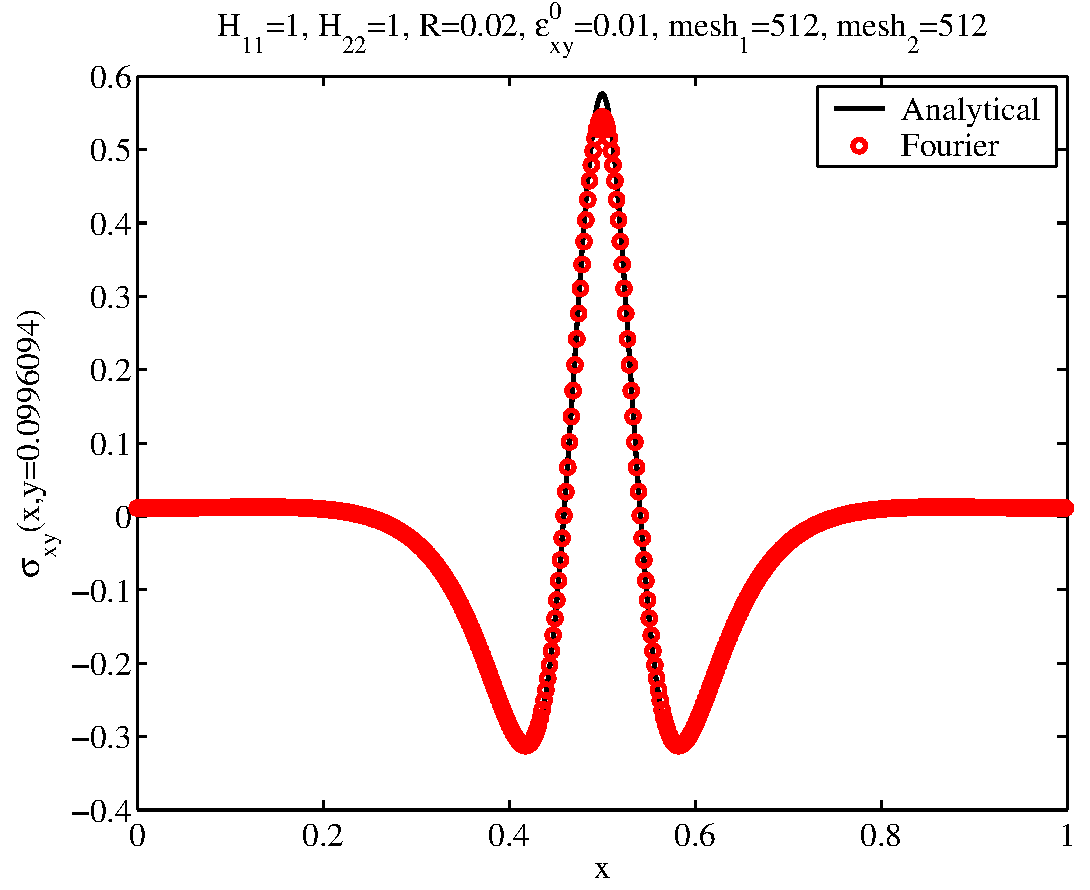
\includegraphics[width=3in]{Figure/CylindricalInclusion}}
\caption{}
\label{CylindricalInclusion}
\end{figure}

Using Mathematica\cite{LiMathematica08} to do the differentiations, we
obtain:
\begin{equation}
 \sigma_{xy}(x,y) \;=\; 
 \frac{\mu \epsilon_{12}^0 R^2(x^4 - 6x^2y^2 + y^4)}{(x^2+y^2)^3(1-\nu)}, \;\;\;\;
 x^2+y^2>R^2
\end{equation}
The comparison with numerical solution is shown in
Fig. \ref{CylindricalInclusion}.


\subsubsection{Sanity Check 4: Cylindrical Void}

Imagine a cylindrical hole of radius $R$ under a far field stress
$\sigma_{ij}^\infty=0$ except $\sigma_{22}^\infty>0$. This is a
plane-strain condition, where $\sigma_{33}(x,y)$ is tuned to make
$\epsilon_{33}(x,y)=0$.  We have non-zero $\epsilon_{11}(x,y)$,
$\epsilon_{22}(x,y)$, $\epsilon_{12}(x,y)$ that must satisfy the
compatibility constraint:
\begin{equation}
 \epsilon_{11,22} + \epsilon_{22,11} \;=\; 2\epsilon_{12,12}.
 \label{PlaneStrainCompatibility}
\end{equation}
There are two stress equilibrium equations:
\begin{equation}
 \sigma_{11,1} + \sigma_{12,2} \;=\; 0, \;\;\;\;
 \sigma_{21,1} + \sigma_{22,2} \;=\; 0
\end{equation}
the finite $\sigma_{33}(x,y)$ is canceled for finite-thickness samples
near the hole exit by 3D indentation like local stress field.  Define
Airy stress function:
\begin{equation}
 \varphi_{,22} \equiv \sigma_{11}, \;\;
 \varphi_{,12} \equiv -\sigma_{12}, \;\;
 \varphi_{,11} \equiv \sigma_{22}
\end{equation}
Stress equilibrium is satisfied. We also have
$\sigma_{33}=\lambda(\epsilon_{11}+\epsilon_{22})$,
$\sigma_{22}=\lambda(\epsilon_{11}+\epsilon_{22})+2\mu\epsilon_{22}$,
$\sigma_{11}=\lambda(\epsilon_{11}+\epsilon_{22})+2\mu\epsilon_{11}$,
so ${\rm tr}(\bmath{\sigma})=(3\lambda+2\mu)(\epsilon_{11}+\epsilon_{22})$, and
based on
(\ref{IsotropicStrainStress}):
\begin{equation}
  \bmath{\epsilon} \;=\; \frac{\bmath{\sigma}}{2\mu} - 
  \frac{\lambda}{2\mu}
 \frac{{\rm tr}(\bmath{\sigma})}{3\lambda+2\mu} {\bf I}.
\end{equation}
Plugging above back into (\ref{PlaneStrainCompatibility}), we get
\begin{equation}
 \nabla^4 \varphi \;=\;
 (\partial_{11}+\partial_{22})(\partial_{11}+\partial_{22}) \varphi
  \;=\;
 (r^{-1}\partial_r(r\partial_r)+r^{-2}\partial_\theta^2)^2 \varphi
 \;=\; 0.
 \label{AiryEquation}
\end{equation}
Converting to cylindrical coordinate, we also have 
\begin{equation}
 \sigma_{rr} = r^{-1}\partial_r\varphi + r^{-2}\partial_\theta^2\varphi, \;\;\;
 \sigma_{\theta\theta} = \partial_r^2 \varphi, \;\;\;
 \sigma_{r\theta} = -\partial_r(r^{-1}\partial_\theta\varphi)
\end{equation}

Since
$\sigma_{22}^\infty=\sigma_{22}(x,y\rightarrow\infty)=\varphi_{,11}(x,y\rightarrow\infty)$,
we see that $\varphi(x,y)$ must contain $\sigma_{22}^\infty x^2/2 =
\sigma_{22}^\infty r^2 \cos^2(\theta)/2 = \sigma_{22}^\infty r^2
(\cos(2\theta)+1)/4$ as the leading-order term.  Presume
$\varphi=r^m g(\theta)$, a $\cos(n\theta)$ angular term excites in
(\ref{AiryEquation}):
\begin{equation}
 0 \;=\; (r^{-1}\partial_r(r\partial_r)-n^2r^{-2})^2 f(r) \;=\;
 r^{m-4}((m-2)^2-n^2)(m^2-n^2),
\end{equation}
which means $m=\pm n, 2\pm n$.  For $n=0$, the solution can be $r^2$, $r^2\ln r$, $1$, $\ln r$.  So
we know the general solution should look like
\begin{equation}
 \varphi \;=\; \frac{\sigma_{22}^\infty}{4}\left[ 
 (r^2 + ar^{-2} + b + 0r^4)\cos(2\theta) + (c\ln r + r^2)\cos(0\theta)
 \right]
\end{equation}
$0r^4$ because we know it does not satisfy the far-field
asymptote. Thus,
\begin{eqnarray}
 \sigma_{rr} =&& r^{-1}\partial_r\varphi + r^{-2}\partial_\theta^2\varphi \nonumber\\
 =&& \frac{\sigma_{22}^\infty}{4} \left[ 
 \cos(2\theta)(r^{-1}(2r-2ar^{-3})-4r^{-2}(r^2 + ar^{-2} + b)) +  r^{-1}(2r+cr^{-1}) \right]
\nonumber\\
 =&& \frac{\sigma_{22}^\infty}{4} \left[ \cos(2\theta) ( -2 - 6ar^{-4} - 4br^{-2} ) + 2 + cr^{-2}
 \right]
\end{eqnarray}
\begin{eqnarray}
 \sigma_{r\theta} =&& -\partial_r(r^{-1}\partial_\theta\varphi) \nonumber\\
 =&& \frac{\sigma_{22}^\infty}{4} \left[ 
 2\sin(2\theta)( \partial_r(r + ar^{-3} + br^{-1} ) ) \right]
\nonumber\\
 =&& \frac{\sigma_{22}^\infty}{4} \left[2\sin(2\theta) (1 - 3ar^{-4} - br^{-2}
 \right]
\end{eqnarray}

To satisfy the traction-free boundary condition:
$0=\sigma_{rr}(r=R,\theta)$, $0=\sigma_{r\theta}(r=R,\theta)$, we
should have: $c=-2R^2$, $1+3aR^{-4}+2bR^{-2}=0$. Also,
\begin{equation}
 1 - 3aR^{-4} - bR^{-2} \;=\; 0
\end{equation}
then $b=-2R^2$, $a=R^4$.  So
\begin{equation}
 \varphi \;=\; \frac{\sigma_{22}^\infty}{4}\left[ 
 \cos(2\theta)(r^2 + R^4r^{-2} - 2R^2) + r^2 - 2R^2\ln r \right]
\end{equation} 
\begin{equation}
 \sigma_{\theta\theta} \;=\; \frac{\sigma_{22}^\infty}{2}\left[ 
 \cos(2\theta)(1 + 3R^4r^{-4}) + 1 + R^2r^{-2}  \right].
\end{equation}
\begin{equation}
 \sigma_{rr} = \frac{\sigma_{22}^\infty}{2} 
\left[ \cos(2\theta) ( -1 - 3R^4r^{-4} + 4R^2r^{-2} ) + 1 - R^2r^{-2}
 \right].
\end{equation}
\begin{equation}
 \sigma_{r\theta} = 
\frac{\sigma_{22}^\infty}{2} \left[\sin(2\theta) (1 - 3R^4r^{-4} + 2R^2 r^{-2})
 \right].
\end{equation}

And 
\begin{eqnarray}
 \sigma_{yy}(x,y) = \sigma_{22}^\infty 
\frac{2(x^2+y^2)^4 + 3R^4(x^4-6x^2y^2+y^4)+R^2(x^6+13x^4y^2+7x^2y^4-5y^6)}{2(x^2+y^2)^4}
\end{eqnarray}

\begin{figure}[th]
\begin{center}
\subfigure[]{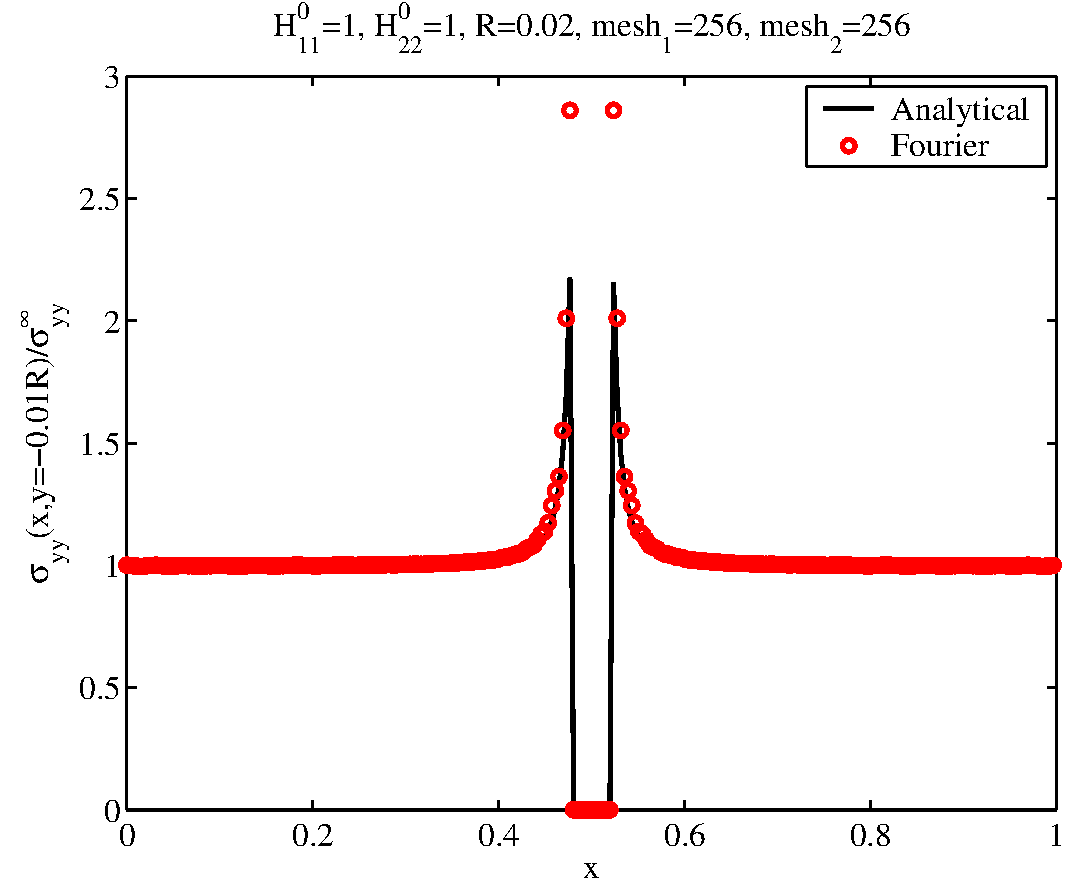
\includegraphics[height=2in]{Figure/CylindricalVoid0}}
\subfigure[]{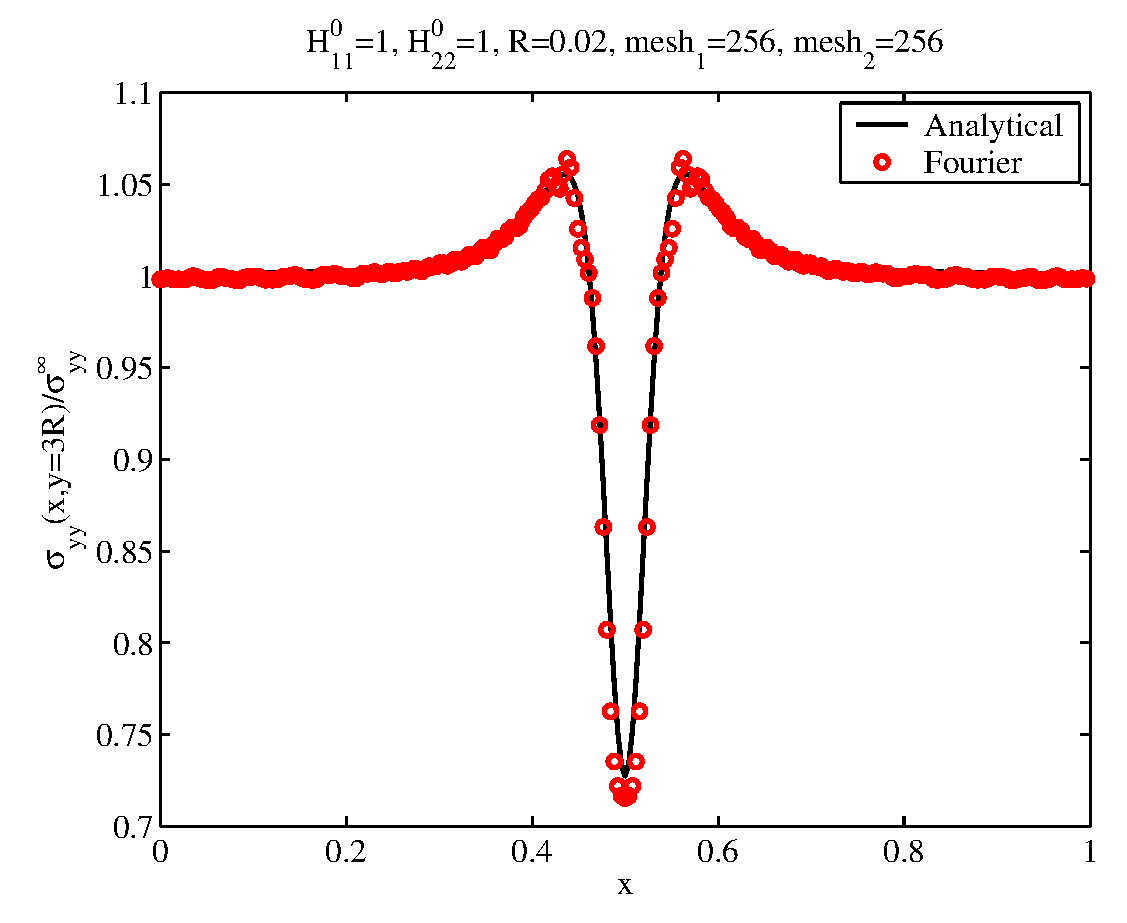
\includegraphics[height=2in]{Figure/CylindricalVoid3}}
\end{center}
\caption{}
\label{CylindricalVoid}
\end{figure}

The above solution is independent of $\nu$ and plane strain vs plane
stress condition.  The only difference between those lies in the
displacement field, not in the stress field.

\bibliography{MyBibliography}
\end{document}
